\documentclass[11pt]{article}

\newcommand{\cnum}{EE 183DA}
\newcommand{\ced}{Winter 2018}
\newcommand{\ctitle}[2]{\title{\vspace{-0.5in}\cnum, \ced\\Lab #1: #2}}
\usepackage{enumitem}
\newcommand{\solution}[1]{{{\color{blue}{\bf Solution:} {#1}}}}
\usepackage[usenames,dvipsnames,svgnames,table,hyperref]{xcolor}
\usepackage{amsmath}
\usepackage{amsfonts}
\usepackage{float}
\usepackage{graphicx}
\usepackage{subcaption}
\usepackage{listings}
\usepackage{color}
\usepackage[bottom]{footmisc}
\usepackage{hyperref}

\hypersetup{
	colorlinks=true,
	linkcolor=blue,
	filecolor=magenta,      
	urlcolor=cyan,
}

\urlstyle{same}

\renewcommand*{\theenumi}{\alph{enumi}}
\renewcommand*\labelenumi{(\theenumi)}
\renewcommand*{\theenumii}{\roman{enumii}}
\renewcommand*\labelenumii{\theenumii.}
\setlist[enumerate,1]{label=(\alph*)}
\setlist[enumerate,2]{label=\theenumii.}

\definecolor{codegreen}{rgb}{0,0.6,0}
\definecolor{codegray}{rgb}{0.5,0.5,0.5}
\definecolor{codepurple}{rgb}{0.58,0,0.82}
\definecolor{backcolour}{rgb}{0.95,0.95,0.92}

\lstdefinestyle{mystyle}{
	backgroundcolor=\color{backcolour},   
	commentstyle=\color{codegreen},
	keywordstyle=\color{magenta},
	numberstyle=\tiny\color{codegray},
	stringstyle=\color{codepurple},
	basicstyle=\footnotesize,
	breakatwhitespace=false,         
	breaklines=true,                 
	captionpos=b,                    
	keepspaces=true,                 
	numbers=left,                    
	numbersep=5pt,                  
	showspaces=false,                
	showstringspaces=false,
	showtabs=false,                  
	tabsize=2
}

\lstset{style=mystyle}

\begin{document}
\ctitle{3-4}{State Estimation and Motion Planning of a Mobile Robot}
\author{Jonathan Chang, Michael Warren, Nick Bruce}
\date{3/13/2018}
\maketitle
\vspace{-0.75in}

\vspace{5mm}

\section{Introduction}

A mobile robot is a common application that requires a multitude of techniques in state estimation, controllability, and motion planning, all which requires contending with noise sensors and forces that cannot be necessarily predicted beforehand. This project uses a robot body printed on paper, so as to minimize the effect of friction, a function of floor material and speed, but the relative looseness in which the electronics sit may have introduced additional noise.

We are given two laser sensors to detect distances at an orthogonal distance, to the front and right, as well as an IMU sensor. For ideal controllability, we would have ideally liked at least 4 range finders at various angles, 2 on each side. For instance, 2 sensors cannot deterministically predict the position of the robot when sensors are pointed at the same wall. Nevertheless, we attempted to contend with the shortcomings of our design. More time would have been preferred to tune parameters and integrate various parts of our road map.

\section{Simulation}

In many projects, physical testing with actual apparatus may be impractical or dangerous. While those are not concerns for this project, simulation, if done right, should reduce time to completion. Therefore, the simulation should be poised to model the reality of the experiment, by using Gaussian noise where necessary and having a proper separation of simulation and model components. We designed our simulation with this in mind.

\begin{figure}[H]
	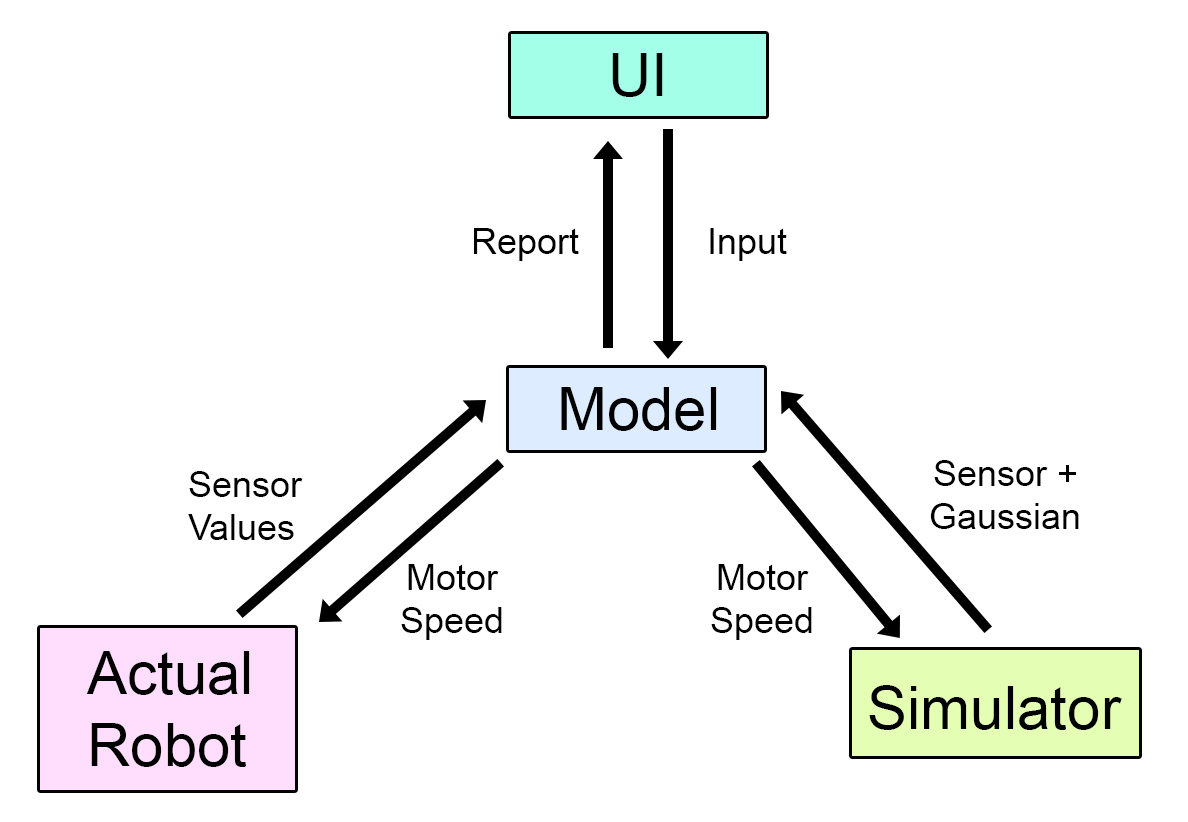
\includegraphics[width=\linewidth]{fig1.png}
	\caption{Organizational flowchart.}
	\label{fig:flow}
\end{figure}

In order to prevent duplicate work, the model should act like an ideal switch, such that trading between the \emph{simulator} and \emph{actual robot} involves minimal preparation. This could be achieved through event programming, and designing a general interface, such that the model itself remains constant regardless of which module passes it sensor values.

\section{User interface}

Although not required for this class, a little bit of design could greatly improve work flow and possibly end results. For example, having a USB cable connected to the robot at all times was something we wanted to avoid, to prevent an extra force affecting end results. We also cannot rely on local network security; therefore, the robot should act as its own access point (although WiFi mode was used for testing). Thankfully, this is a feature on the \emph{ESP8266}. A combination of Javascript and Python was chosen for their browser integration without much work, such that we could have a good reporting and controlling scheme for feedback purposes.

\begin{figure}[H]
	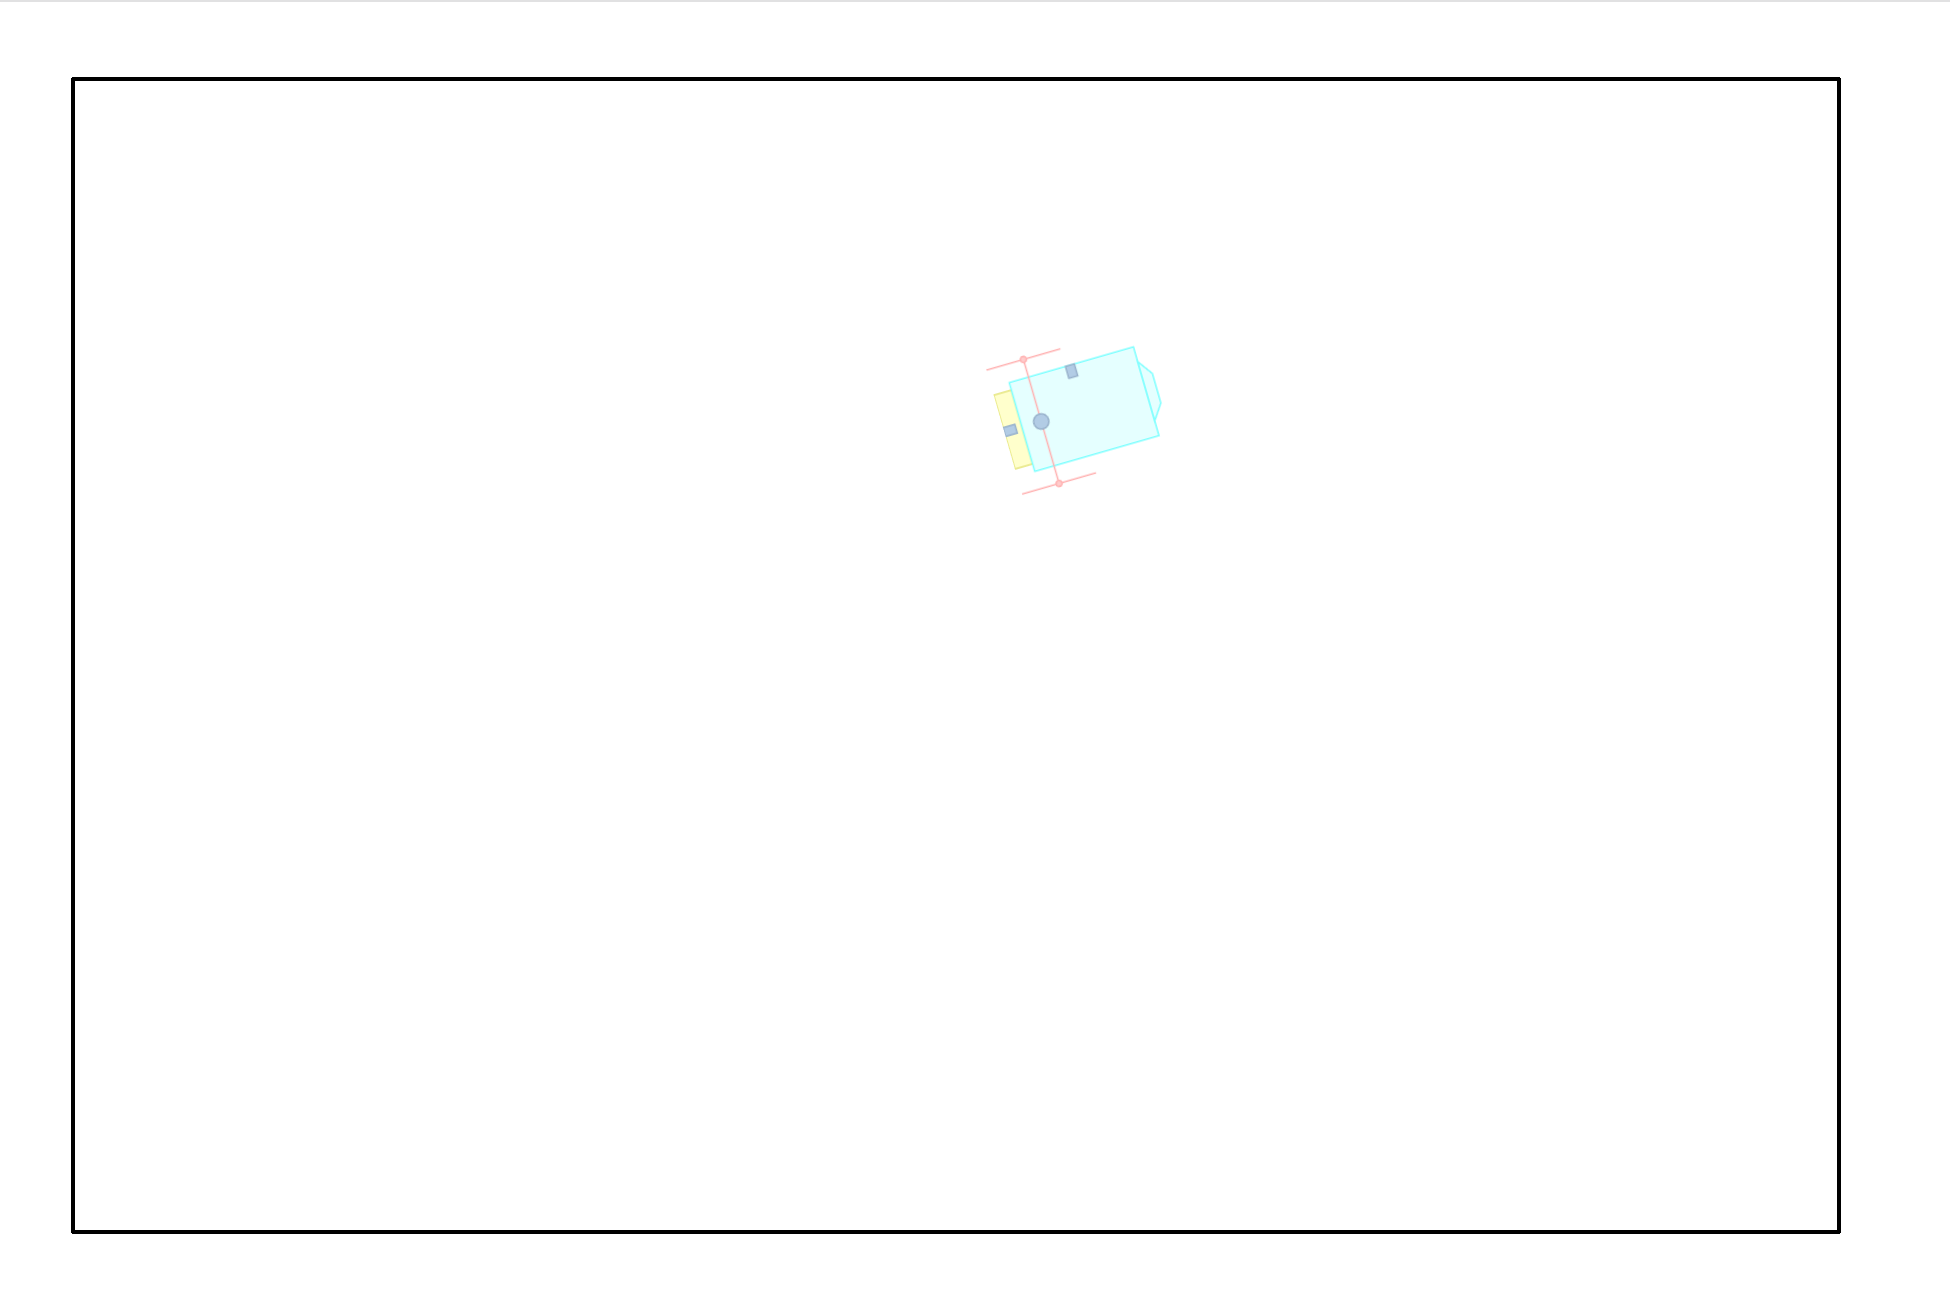
\includegraphics[width=\linewidth]{fig1a.png}
	\caption{Used to test estimation iterations with keyboard.}
	\label{fig:uisim}
\end{figure}

\section{Model}

To model the simulation, we use the \emph{Extended Kalman Filter (EKF)}, since we have a non-linear function. The EKF requires various parameters, such as noise and variance matrices, that may be hard to determine, whether experimentally or mathematically. The observational matrix, $R$, could be determined by measuring noise without input at start, or consulting sensor specifications. For example, a glance through documention finds

 \begin{table}[H]
	\begin{tabular}{|c|c|}
		
		\hline
		sensor & notes \\
		\hline\hline
		Adafruit GY VL53LOX Laser sensors & 0.03-0.12 ranging accuracy error. \\ \hline
		FEETECH FS90R Continuous servo & 100-130 max rpm, no load. \\ \hline
		MPU-9250 & $\pm 0.005$ non-linearity. \\
		\hline
		
	\end{tabular}
	\caption{Sensor errors and limits}\label{table:errlim}
\end{table}



\section{Estimate state}

The \emph{Extended Kalman Filter (EKF)} prediction step requires that

\begin{equation}
\hat{x}_t = f(x_{t-1}, u_t, w_t)
\end{equation}

We use the previous state, which comprises $\left[x, y, \theta, v\right]$, and sensors as inputs. The sensors are $a$, the acceleration in the forward direction in robot frame of reference measured by the accelerometer; and $\dot{\theta}$, the change in angle since the last reading measured by the gyro.

By approximation, the arc length,
\begin{equation}
\alpha \approx \frac{v + a}{2}
\end{equation}

Since $\alpha = r \dot{\theta}$, the turn radius,
\begin{equation}
r = \frac{\alpha}{\dot{\theta}}
\end{equation}

To prevent large calculations approaching infinite, and division by zero errors, we consider two cases separately. If $\dot{\theta} > 0.1$, we consider that the robot is turning. Otherwise, the robot is going relatively straight.

If the robot is turning, we need to find the center of rotation. We know the $r$ and $\alpha$, so we apply a transform to find the point a distance of $r$ to the right relative to the robot state. This is a rotation of the relative position $-r$ by $\theta$, then a translation by $x$ and $y$. The result is
\begin{equation}
p_{center} = \begin{bmatrix}
-r cos\theta + x \\ -r sin\theta + y
\end{bmatrix}
\end{equation}

We must then rotate by $\alpha$ about $p_{center}$. By applying the transformation matrix again, we end up in
\begin{equation}
p_{new} = \begin{bmatrix}
r cos\theta cos\dot{\theta} - rsin\theta sin\dot{\theta} - r cos\theta + x \\
r sin\theta cos\dot{\theta} + r sin\dot{\theta} cos\theta - r sin\theta + y
\end{bmatrix}
\end{equation}

By trigonometric identities,
\begin{equation}
p_{new} = \begin{bmatrix}
r (cos(\theta + \dot{\theta}) - cos\theta) + x \\
r (sin(\theta + \dot{\theta}) - sin\theta) + y
\end{bmatrix}
\end{equation}

On the other hand, if the robot goes nearly straight, then a transformation matrix with the original position as origin, and the robot travels by some $\alpha$ leaves
\begin{equation}
p_{new} = \begin{bmatrix}
-\alpha sin\theta + x \\
\alpha cos\theta + y
\end{bmatrix}
\end{equation}

In either case,
\begin{align}
\theta_{new}  & = \theta + \dot{\theta} \\
v_{new} & = v + a
\end{align}

Therefore, in the turning condition, the state estimation matrix Jacobian becomes
\begin{equation}
A = \begin{bmatrix}
\frac{\partial f_x}{\partial x} & \frac{\partial f_x}{\partial y} & \frac{\partial f_x}{\partial \theta} & \frac{\partial f_x}{\partial v} \\
\frac{\partial f_y}{\partial x} & \frac{\partial f_y}{\partial y} & \frac{\partial f_y}{\partial \theta} & \frac{\partial f_y}{\partial v} \\
\frac{\partial f_{\theta}}{\partial x} & \frac{\partial f_{\theta}}{\partial y} & \frac{\partial f_{\theta}}{\partial \theta} & \frac{\partial f_{\theta}}{\partial v} \\
\frac{\partial f_v}{\partial x} & \frac{\partial f_v}{\partial y} & \frac{\partial f_v}{\partial \theta} & \frac{\partial f_v}{\partial v}
\end{bmatrix}
\end{equation}

The equations are
\begin{align}
\frac{\partial f_x}{\partial x} & = 1 \\
\frac{\partial f_x}{\partial y} & = 0 \\
\frac{\partial f_x}{\partial \theta} & = r(sin\theta - sin(\theta + \dot{\theta})) \\
\frac{\partial f_x}{\partial v} & = \frac{cos(\theta + \dot{\theta}) - cos\theta}{2 \dot{\theta}} \\
\frac{\partial f_y}{\partial x} & = 0 \\
\frac{\partial f_y}{\partial y} & = 1 \\
\frac{\partial f_y}{\partial \theta} & = r(cos(\theta + \dot{\theta}) - cos\theta) \\
\frac{\partial f_y}{\partial v} & = \frac{sin(\theta + \dot{\theta}) - sin\theta}{2 \dot{\theta}} \\ 
\frac{\partial f_{\theta}}{\partial x} & = \frac{\partial f_{\theta}}{\partial y} = \frac{\partial f_{\theta}}{\partial v} = 0 \\
\frac{\partial f_{\theta}}{\partial \theta} & = 1 \\
\frac{\partial f_v}{\partial x} & = \frac{\partial f_v}{\partial y} = \frac{\partial f_v}{\partial \theta} = 0 \\
\frac{\partial f_v}{\partial v} & = 1
\end{align}

In a straight line, the equations are
\begin{align}
\frac{\partial f_x}{\partial x} & = 1 \\
\frac{\partial f_x}{\partial y} & = 0 \\
\frac{\partial f_x}{\partial \theta} & = 0 \\
\frac{\partial f_x}{\partial v} & = \frac{-cos\theta}{2} \\
\frac{\partial f_y}{\partial x} & = 0 \\
\frac{\partial f_y}{\partial y} & = 1 \\
\frac{\partial f_y}{\partial \theta} & = 0 \\
\frac{\partial f_y}{\partial v} & = \frac{sin\theta}{2} \\
\frac{\partial f_{\theta}}{\partial x} & = \frac{\partial f_{\theta}}{\partial y} = \frac{\partial f_{\theta}}{\partial v} = 0 \\
\frac{\partial f_{\theta}}{\partial \theta} & = 1 \\
\frac{\partial f_v}{\partial x} & = \frac{\partial f_v}{\partial y} = \frac{\partial f_v}{\partial \theta} = 0 \\
\frac{\partial f_v}{\partial v} & = 1
\end{align}
\newpage

We can also describe an input Jacobian matrix, such that
\begin{equation}
B = \begin{bmatrix}
\frac{\partial f_x}{\partial \dot{\theta}} & \frac{\partial f_x}{\partial a} \\
\frac{\partial f_y}{\partial \dot{\theta}} & \frac{\partial f_y}{\partial a} \\
\frac{\partial f_\theta}{\partial \dot{\theta}} & \frac{\partial f_\theta}{\partial a} \\
\frac{\partial f_v}{\partial \dot{\theta}} & \frac{\partial f_v}{\partial a}
\end{bmatrix}
\end{equation}

In the turning condition, the equations are
\begin{align}
\frac{\partial f_x}{\partial \dot{\theta}} & = -\frac{v+a}{2 \dot{\theta}^2} (cos(\theta + \dot{\theta}) - cos\theta) - \frac{v+a}{2 \dot{\theta}} sin(\theta + \dot{\theta}) \\
\frac{\partial f_x}{\partial a} & = \frac{1}{2 \dot{\theta}} (cos(\theta + \dot{\theta}) - cos\theta) \\
\frac{\partial f_y}{\partial \dot{\theta}} & = -\frac{v+a}{2 \dot{\theta}^2} (sin(\theta + \dot{\theta}) - sin\theta) + \frac{v+a}{2 \dot{\theta}} cos(\theta + \dot{\theta}) \\
\frac{\partial f_y}{\partial a} & = \frac{1}{2 \dot{\theta}} (sin(\theta + \dot{\theta}) - sin\theta) \\
\frac{\partial f_{\theta}}{\partial \dot{\theta}} & = 1 \\
\frac{\partial f_{\theta}}{\partial a} & = 0 \\
\frac{\partial f_v}{\partial \dot{\theta}} & = 0 \\
\frac{\partial f_v}{\partial a} & = 1 
\end{align}

In a straight line,
\begin{align}
\frac{\partial f_x}{\partial \dot{\theta}} & = 0 \\
\frac{\partial f_x}{\partial a} & = \frac{-cos\theta}{2} \\
\frac{\partial f_y}{\partial \dot{\theta}} & = 0 \\
\frac{\partial f_y}{\partial a} & = \frac{sin\theta}{2} \\
\frac{\partial f_{\theta}}{\partial \dot{\theta}} & = 0 \\
\frac{\partial f_{\theta}}{\partial a} & = 1 \\
\frac{\partial f_v}{\partial \dot{\theta}} & = 1 \\
\frac{\partial f_v}{\partial a} & = 0 
\end{align}

$w$ is a time invariant value.

\section{Estimate state by input}

Similarly, given left and right inputs, we could define the motor speed as approximately
\begin{align}
V_L = \gamma_{i, L} * V_{max} \\
V_R = \gamma_{i, R} * V_{max}
\end{align}

where $V_{max}$ is some function of the maximum $RPM$ found in the specs, and $\gamma_i$ are ratios of inputs over the maximum allowable value. Suppose that turning left is the positive angle, and let $r$ be the turn radius of the left wheel and $w$ be the width of the robot, then
\begin{equation}
\begin{split}
\frac{V_L}{r} & = \frac{V_R}{r+w} \\
\frac{r+w}{r} & = \frac{V_R}{V_L} \\
\frac{w}{r} & = \frac{V_R - V_L}{V_L} \\
r & = \frac{V_L w}{V_R - V_L}
\end{split}
\end{equation}

The radius from the center of the robot is
\begin{equation}
\begin{split}
r* & = w \left(\frac{V_R}{V_R - V_L} + \frac{1}{2}\right) \\
& = w \left(\frac{V_L + 0.5(V_R - V_L)}{V_R - V_L}\right) \\
& = \frac{w}{2} \left(\frac{V_R + V_L}{V_R - V_L}\right)
\end{split}
\end{equation}

Since arc length at the center of the robot is
\begin{equation}
\alpha = \frac{V_R + V_L}{2}
\end{equation}

the change in angle is
\begin{equation}
\begin{split}
\dot{\theta} & = \frac{\alpha}{r*} \\
& = \frac{V_R - V_L}{w}
\end{split}
\end{equation}

With $r$, $\alpha$, $\theta$, $\dot{\theta}$, $x$, and $y$, we proceed with the rest of the calculations as the same as before, by finding the center and then rotating about it using the rotation and translation matrices.

\section{Estimate covariance}

Covariance estimate is
\begin{equation}
P_t = A P_{t-1} A + B \Gamma_{t-1} B + Q
\end{equation}

Since the actual state is unknown, the state covariance matrix is initialized as identity,
\begin{equation}
P_0 = \begin{bmatrix}
1 & 0 & 0 & 0 \\
0 & 1 & 0 & 0 \\
0 & 0 & 1 & 0 \\
0 & 0 & 0 & 1
\end{bmatrix}
\end{equation}

Input covariance is also unknown, so we scale the input covariance matrix by the maximum value of input so that its relative weight is accurate. For the gyro, maximum $rpm$ is about $100$, with some load assumed; therefore, given that axle length is $8.4cm$ and wheel circumference is $\pi * 4.9cm$, it can make a full circle in a $ms$. $\dot{\theta}_{max} \approx 0.001*\mathrm{(period)}$. Given $100 rpm$, the maximum speed is about $0.0257cm/ms$. The acceleration can be limited by the control algorithm. We can assume that the maximum is a tenth, making $\dot{v}_{max} \approx 0.00257*\mathrm{(period)}$.

\begin{equation}
\Gamma = \begin{bmatrix}
0.00101 & 0 \\
0 & 0.00257
\end{bmatrix}
\end{equation}

\section{Innovation}

In the innovation step, we measure the actual state such that 

\begin{equation}
z_t = h(\hat{x}_t, v_t) + y
\end{equation}

where $y$ is the residual.

$v_t$ depends on the variances of the sensors. $h$ depends on the wall that the laser sensors projects on. Using the estimated state $\hat{x}_t$, we calculate for the wall of shortest distance by the quadrant under which the sensors face. The quadrant was found to be

\begin{equation}
\begin{split}
p & =\mathrm{floor}\left[\frac{\theta}{\pi / 4}\right] + 2 \\
map & = [4, 1, 2, 3] \\
q & = p[map]
\end{split}
\end{equation}  

Depending on the wall the sensors project on, we can determine either $x$ or $y$. Therefore, if the two sensors project on adjacent walls, a position is absolutely determinable. Otherwise, we need to fuse it with the a projection from the estimated state. Let $f$ and $r$ be the distance measurements, and $h$ and $w$ be height and width respectively. Then, for the front sensor

 \begin{table}[H]
 	\centering
	\begin{tabular}{|c|c|c|}
		\hline
		wall & position & $\delta\theta$ \\
		\hline\hline
		front & ($f sin\theta$, ? ) & ($f cos\theta$, ? ) \\ \hline
		top & (?, $h - f cos\theta$) & (?, $f sin\theta$) \\ \hline
		left & ($w + f sin\theta$, ? ) & ($f cos\theta$, ? ) \\ \hline
		bottom & (?, $-f cos\theta$) & (?, $f sin\theta$) \\ \hline
	\end{tabular}
	\caption{Positions determined by front sensor.}\label{table:fpos}
\end{table}
\newpage
For the right sensor

 \begin{table}[H]
 	\centering
	\begin{tabular}{|c|c|c|}
		\hline
		wall & position & $\delta\theta$ \\
		\hline\hline
		front & ($-rcos\theta$, ? ) & ($r sin\theta$, ? ) \\ \hline
		top & (?, $h - f sin\theta$) & (?, $-r cos\theta$) \\ \hline
		left & ($w -r cos\theta$, ? ) & ($r sin\theta$, ? ) \\ \hline
		bottom & (?, $-f sin\theta$) & (?, $-r cos\theta$) \\ \hline
	\end{tabular}
	\caption{Positions determined by right sensor}\label{table:rpos}
\end{table}

We take an average measured by the two sensors, if the axis repeats, and fill in the unknown values by projecting from the estimated state.

\section{Kalman gain}

To complete the update step, we must find the Kalman gain. First, we find the residual $y$ by computing the differences between the measured and estimated states. Then, the steps are

\begin{align}
S & = HPH^T + R \\
K & = \frac{PH^T}{S} \\
x & = \hat{x} + Ky \\
P_t & = (I - KH) P_{t-1}
\end{align}

\section{Finding initial conditions}

While it is possible to place the robot in a predetermined location at each trial, this introduces human error and makes the system less robust. It is useful to have a procedure in which the robot could determine initial conditions. We use a \emph{variation of angles} method to calibrate. The steps are

\begin{enumerate}
\item[1.] We measure the initial distance from the front sensor and angle.
\item[2.] We turn by some small known $\delta \theta$.
\item[3.] We measure a second distance $f_2$ from the front sensor and angle $\theta_2$.
\item[4.] We calculate the least angle along the current wall and go back to it.
\item[5.] We turn 180$\deg$ and measure the opposite site.
\end{enumerate}

By calibrating as such, we could also estimate observation noise, and angle at shortest distances to determine the box size, and box orientation from magnetic North.

Calculation involves basic trigonometric facts. We assume in most circumstances, turning a small angle allows the robot to project on the same wall. Therefore, let $\delta \theta = \theta_2 - \theta_1$ as measured by the magnetometer. Using the law of cosines,

\begin{equation}
x^2 = f_1^2 + f_2^2 - 2 f_1 f_2 cos\delta\theta
\end{equation}

where $x$ denotes the length of wall between the two angles. Now, using the law of sines, we note that

\begin{equation}
\frac{x}{sin\delta\theta} = \frac{f_1}{\beta}
\end{equation}

where $\beta$ is the angle $\angle_{f_2, wall}$. Note that this angle must form a right angle between the point where the second laser projects on the wall, the robot, and the point of least distance, such that the ideal angle

\begin{equation}
\hat{\theta} = |90 - \beta|
\end{equation}

The sign of $\hat{\theta}$ determines whether the robot has to travel back or forward to find this angle. We measure $\hat{f_1}$ and $\hat{r_1}$ at $\hat{\theta}$, and $\hat{f_2}$ and $\hat{r_2}$ at $\hat{\theta + \pi}$, such that the width of the box is $\hat{f_1} + \hat{f_2} + 2d$, where $d$ is the distance between the front sensor and the center of the robot axle. The complementary angles are the same, except with the right sensor.

\section{Motion Planning}

With a decent state representation, we send the robot a state and target value, and the robot performs a \emph{rapidly exploring random tree} algorithm to find the target. An $x$-$y$ plot of the robot converging on the target is shown

\begin{figure}[H]
	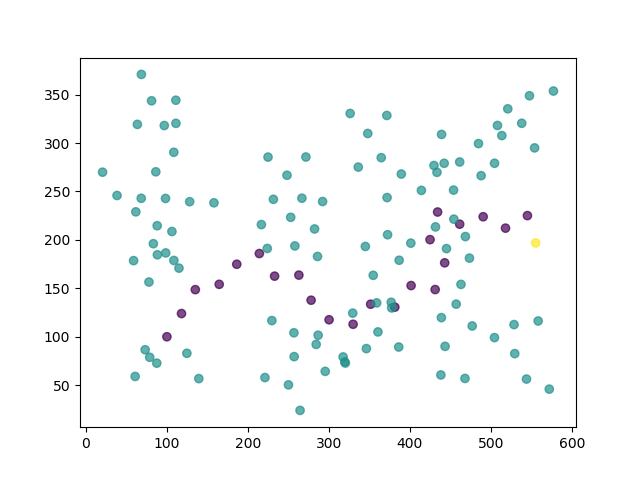
\includegraphics[width=\linewidth]{fig2.png}
	\caption{Rapidly-exploring random tree convergence.}
	\label{fig:rrt}
\end{figure}

The algorithm works by generating a random configuration tree, then selecting vertices that are incrementally closer to the target.

\section{Code}

For complete code, see

	\href{https://github.com/jachang820}{https://github.com/jachang820}
	
In particular, note these directories:

	\href{https://github.com/jachang820/Mobile-Robot-Simulator/tree/master/mysite/simulation/static/js}{Model, simulation}
	
	\href{https://github.com/jachang820/Mobile-Robot-Simulator/tree/master/arduino}{Code on the robot}

\end{document}
